
\begin{figure*}
	\centering
		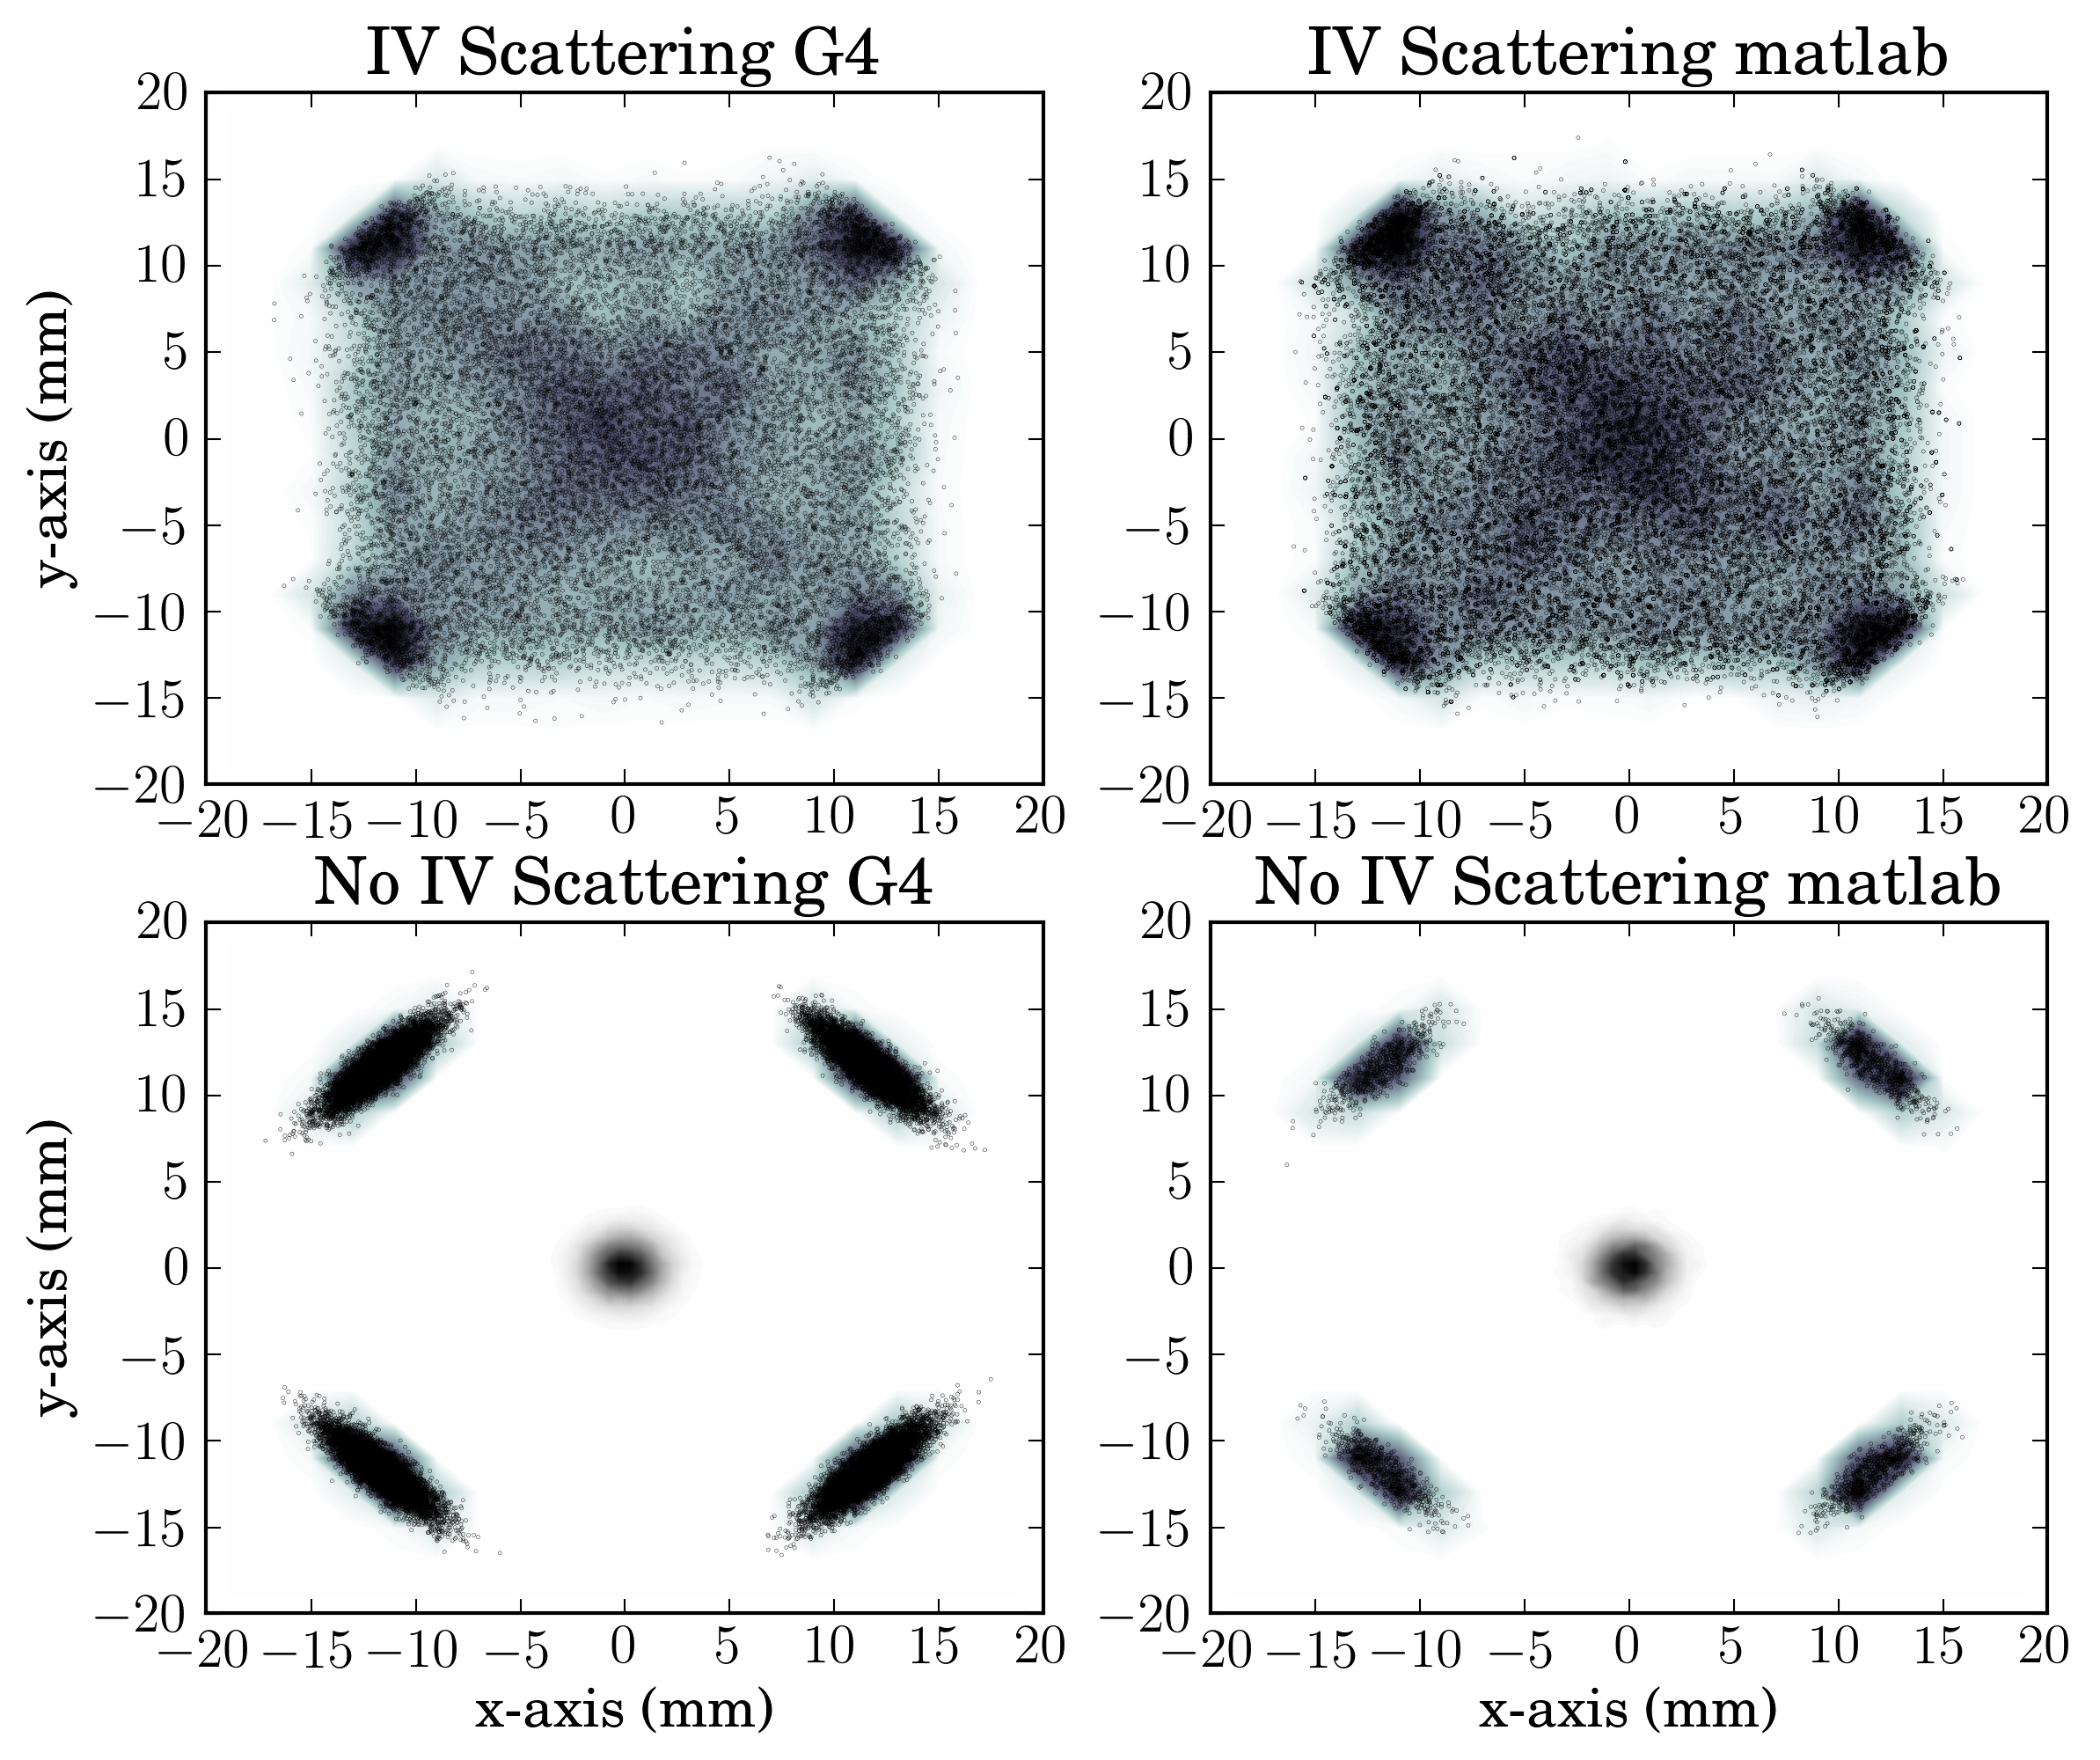
\includegraphics[width=0.9\textwidth]{intervalley.png}
	\caption{\textbf{Left:} Geant4 simulations \textbf{Right:} legacy MATLAB simulations. \textbf{Top Row:} Simulations with inter-valley scattering turned on, \textbf{Bottom Row:} Simulations with inter-valley scattering turned off, including hole transport through the crystal.}
	\label{fig:intervalley}
\end{figure*}

Electron propagation as discussed in the previous section, has one particularly interesting feature that electrons propagate through the crystal in one of four distinct valleys \cite{Cabrera,Leman}. Electrons are not bound to those valleys permanently, however, and can scatter between valleys. This process is known as inter-valley scattering and occurs in one of two ways: 1. an electron scatters of the lattice or 2. of an impurity in the crystal structure \cite{iv}. The rate for both processes is dependent on the electric field strength with lattice scattering being the dominant factor in larger fields ($\gtrsim$5~V/m), while impurity scattering dominates in lower fields ($\sim$1~V/m). The EDELWEISS \cite{edelweiss} collaboration determined the scattering rates as a function of the electric field for typical Ge crystals \cite{iv}. We use the results obtained in these studies to set the inter-valley scattering amplitude in the Geant4 framework and compare it to previous implementations of the charge transport 
code \cite{Cabrera,Leman}. The result of electrons and holes propagating through 2.54~cm of Ge in an 0.5~V/m electric field is shown in Figure~\ref{fig:intervalley}. The top two panels show the result with inter-valley scattering turned on while the bottom two panels show the result for inter-valley scattering turned off. The panels on the right show the results for the legacy simulation \cite{Cabrera,Leman} with somewhat less statistics than the Geant4 simulations. The bottom two panels also show the hole transport through the crystal for the G4 and legacy simulations \cite{Cabrera,Leman}. 
